Per distillazione si intende la tecnica utilizzata per separare due o più sostanze presenti in una miscela. Essa sfrutta la differenza dei punti di ebollizione di tali sostanze, cioè la loro differenza di volatilità.
\subsection{La legge di Raoult}
\subsubsection{DEF. Soluzione ideale}
Supponiamo di avere due liquidi in soluzione, ad esempio alcol etilico e acqua. Diciamo che questa soluzione è \textit{ideale} se per i due liquidi, i quali devono essere totalmente miscibili cioè A si scioglie totalmente in B o viceversa B si scioglie totalmente in A qualunque siano le proporzioni, il $\Delta$H di mescolamento è pari a zero.

Di norma il $\Delta$H è diverso da zero, ma spesso si lavora con soluzioni diluite e pertanto le condizioni in cui lavoriamo sono prossime all'idealità.

\vspace{0.2cm}I liquidi hanno la caratteristica di evaporare, ed è evidente che se evaporano avremo particelle di A e di B in fase vapore. Nelle condizioni di idealità dei gas sappiamo che ogni specie gassosa si comporta come se fosse l'unica presente nel contenitore, pertanto se sia il vapore di A che quello di B viene assimilato ad un gas ideale ognuno dei due si comporterà come se fosse l'unico presente e quindi la pressione totale potrà essere calcolata come somma delle pressioni parziali dei componenti A e B:
$$P=P_A + P_B \quad \text{(Legge di Dalton)}$$
Ovviamente stiamo immaginando di trovarci ad una data temperatura, cioè fissiamo una temperatura alla quale troviamo una certa pressione/tensione di vapore dovuta al componente A e un'altra dovuta al componente B e la cui somma dà la pressione totale.

Se non avessimo questa soluzione, quale sarebbe la tensione di vapore di ognuna delle due speci pure? 

Innanzitutto indichiamo con $P^0_A$ e $P^0_B$ le tensioni di vapore di ognuno dei due liquidi pure alla temperatura $T$ alla quale stiamo lavorando. Quindi, fissata la temperatura, il componente A eserciterà la pressione $P^0_A$ se puro, mentre se è in miscela eserciterà la pressione $P_A$. Analogamente per il componente B.

Qual è la relazione tra $P^0_A$ e $P_A$?

La loro relazione è data dalle \textit{legge di Raoult}, la quale dice che la tensione di vapore di un componente in soluzione ad una data temperatura $T$ è pari alla tensione di vapore di quel componente puro alla stessa temperatura, moltiplicata per la sua frazione molare:
$$P_A=\rchi_A P^0_A \qquad P_B=\rchi_B P^0_B \quad \text{Legge di Raoult}$$
Va da ricordare che la frazione molare di ogni componente è sempre inferiore a 1, per cui si ha sempre $P_A < P^0_A$. Quindi si ha un abbassamento delle tensioni di vapore delle singole speci quando le mettiamo in soluzione.

Inoltre, al variare della composizione della miscela variano anche le frazioni molari e di conseguenza varieranno $P_A$ e $P_B$, ma in generale la pressione sarà sempre data da
$$P=\rchi_A P^0_A + \rchi_B P^0_B$$
Ovviamente per calcolarla dovremo fissare temperatura e composizione.

Va da notare che $\rchi_A$ e $\rchi_B$ sono le frazioni molari in soluzione, mentre con questo metodo abbiamo calcolato la pressione del vapore. Allora quale sarà la composizione del vapore alla stessa temperatura?

Intuitivamente possiamo dire che nella fase vapore avremo più abbondanza del componente più volatile\footnote{la volatilità è la tendenza delle sostanze liquide o solide a passare allo stato di vapore.}. Dobbiamo però quantificare.

Abbiamo supposto che la soluzione sia ideale, per cui i vapori si comporteranno idealmente, cioè come se ognuno di loro fosse l'unico ad occupare l'intero volume a disposizione.

Se trattiamo i vapori come gas ideali avremo

$$P_AV=n_ART
\qquad
P_BV=n_BRT$$

Sommiamo le espressioni:

$$(P_A + P_B)V= (n_A + n_B)RT$$

Dalla legge di Dalton sappiamo che la somma delle pressioni parziali è pari alla pressione totale:

$$P=P_A + P_B \implies PV=(n_A + n_B)RT$$

Questa espressione ci permette di avere informazioni sulla fase vapore. Tuttavia adesso $n_A$ e $n_B$ non sono le moli in soluzione, ma le moli in fase vapore.

Dividiamo entrambe le espressioni per quest'ultima:

$$\frac{P_AV}{PV}= \frac{n_ART}{(n_A + n_B)RT}
\implies
\frac{P_A}{P} = \frac{n_A}{n_A + n_B}\equiv \rchi '_A
\implies
P_A=P \cdot \rchi '_A$$

Questa sarà la frazione molare di A in fase vapore. Un risultato analogo si ottiene per B: $P_b=P \cdot \rchi '_B$.

Esplicitando P si otterrà
$$\rchi '_A=\frac{P_A}{P}=
\frac{P_A}{\rchi_A P_A^0 + \rchi_B P_B^0}=
\frac{\rchi_A P_A^0}{\rchi_A P_A^0 + \rchi_B P_B^0}$$

$$\rchi '_B=\frac{P_B}{P}=
\frac{P_B}{\rchi_A P_A^0 + \rchi_B P_B^0}=
\frac{\rchi_B P_B^0}{\rchi_A P_A^0 + \rchi_B P_B^0}$$
Questi calcoli sono necessari in quanto di norma il vapore non avrà la stessa composizione della soluzione a meno che vengano usati due liquidi con la stessa volatilità, cioè con la stessa temperatura di ebollizione.

A questo punto riscriviamo le equazioni delle frazioni molari in fase vapore dividendo numeratore e denominatore rispettivamente per $P_A^0$ e $P_B^0$:
$$\rchi'_A=\frac{\rchi_A}{\rchi_A + \rchi_B\frac{P^0_B}{P^0_A}}
\qquad
\rchi'_B=\frac{\rchi_B}{\rchi_A\frac{P^0_B}{P^0_A} + \rchi_B}$$
In questo modo abbiamo delle relazioni tra frazioni molari in fase vapore e frazioni molari in soluzione.

Per definizione la somma delle frazioni molari è pari a 1, cioè $\rchi_A + \rchi_B =1$. Si avranno allora tre casi:
\begin{itemize}
    \item $P_A^0=P_B^0$, cioè i due liquidi hanno la stessa tensione di vapore. Allora dalle espressioni precedenti avremo che $\rchi_A'=\rchi_A$ e $\rchi_B'=\rchi_B$, ossia la composizione del vapore è identica a quella della soluzione, in quanto stessa tensione di vapore implica stessa volatilità;
    \item $P_B^0>P_A^0$, cioè a parità di temperatura la tensione di vapore del liquido puro B è maggiore di quella del liquido puro A. Ne segue che B è più volatile e in fase vapore ne troviamo di più.
    
    In questo caso $\frac{P_B^0}{P_A^0}>1$, per cui $\big[\rchi_A + \rchi_B\left(\frac{P_B^0}{P_A^0}\right)\big]>1$ e quindi $\rchi_A' < \rchi_A$ e in modo analogo $\rchi_B' > \rchi_B$, cioè essendo B più volatile la composizione del vapore sarà più ricca in B e meno in A.
    \item  $P_A^0>P_B^0$, cioè a parità di temperatura A è più volatile, quindi stavolta il vapore sarà più ricco nel componente A nonostante la composizione della soluzione.
    
    Si avrà quindi $\rchi_A' > \rchi_A$ e $\rchi_B' < \rchi_B$,
\end{itemize}

Consideriamo adesso un grafico in cui, fissata la temperatura, abbiamo in ascissa la frazione molare e nelle ordinate la tensione di vapore:

\begin{minipage}{0.4\textwidth}
    \begin{figure}[H]
        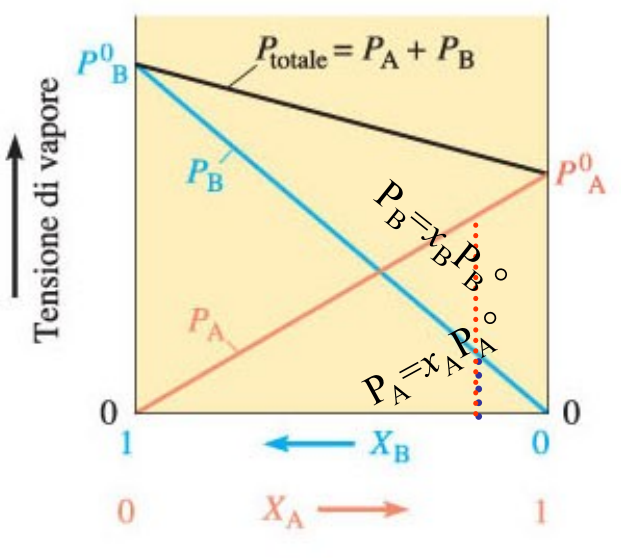
\includegraphics[width=6cm]{immagini/tensione_di_vapore_sol_ideale.png}
    \end{figure}
\end{minipage}
\begin{minipage}{0.6\textwidth}
    Nell'origine avremo il 100\% di B mentre A è assente (0\%). Man mano che ci spostiamo lungo le ascisse aumenta A, fino ad arrivare al punto opposto in cui abbiamo lo 0\% di B e il 100\% di A. Ovviamente la frazione molare è data in numeri, quindi negli estremi una vale 1 e l'altra vale 0.

    Per quanto riguarda le ordinate, nel punto in cui si ha il 100\% di B avremo la tensione di vapore di B puro, cioè $P^0_B$, mentre nel punto opposto in cui abbiamo solo A avremo la tensione di vapore del liquido A puro, cioè $P^0_A$.
\end{minipage}

Le due linee oblique rosse e blu rappresentano tutte le possibili tensioni di vapore di ognuno dei componenti al variare della composizione della miscela. La linea nera rappresenta la somma di tutte le possibili pressioni totali, ottenute sommando le ordinate.

Tale grafico è valido solo se la soluzione è ideale, cioè se il $\Delta$H di mescolamento è pari a zero, ossia è valido se siamo nel campo di validità della legge di Raoult.

\vspace{0.2cm}E se invece la soluzione non è ideale, cioè se mostra un $\Delta$H di mescolamento diverso da zero?

Le soluzioni ideali sono rare, per cui di norma si hanno comportamenti che derivano delle legge di Raoult.

Va da ricordare che l'obiettivo è quello di conoscere la termodinamica di queste soluzioni per poterla sfruttare per separare la soluzione nei suoi componenti. Ci è quindi utile conoscere la composizione del vapore per poterlo trattare col fine di arrivare ad una composizione diversa (separandolo dal liquido e condensandolo). Ad esempio in una soluzione di acqua e alcol non è possibile separare per distillazione acqua e alcol: si arriva ad un certo punto e poi non si riesce più. Dobbiamo capire perché.

\vspace{0.2cm}\textbf{Processo di solubilizzazione endotermico}

Immaginiamo che il $\Delta$H sia diverso da zero, ad esempio maggiore di zero. Ciò significa che il sistema sta assorbendo calore, ossia per potere sciogliere A e B dobbiamo riscaldare, cioè dobbiamo fornire energia altrimenti la soluzione non si forma. Ciò capita tutte le volte in cui le interazioni che verranno a formarsi tra A e B sono più deboli di quelle che esistono nei liquidi puri, ovvero le interazioni A-A e B-B (per formare una soluzione si devono separare le particelle di soluto e quelle di solvente. Separare significa rompere le interazioni che si esercitano tra i componenti puri, cioè tra le loro molecole). 

\vspace{-0.3cm}\begin{minipage}{0.4\textwidth}
    \begin{figure}[H]
        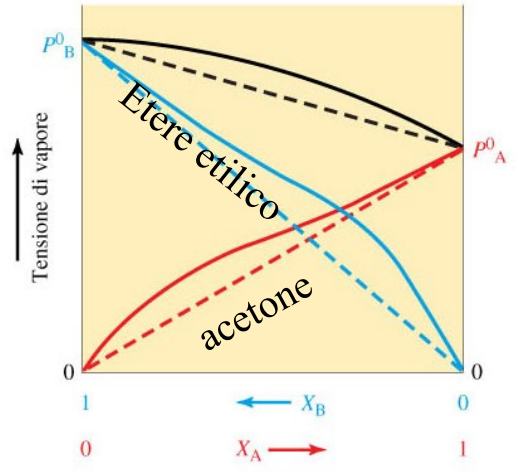
\includegraphics[width=6cm]{immagini/tensione_di_vapore_sol_endotermica.png}
    \end{figure}
\end{minipage}
\begin{minipage}{0.6\textwidth}

\vspace{0.4cm}In questo grafico e linee tratteggiate indicano il comportamento ideale, quelle continue descrivono il comportamento sperimentale, ottenuto misurando la tensione di vapore con varie composizioni.

Siccome le interazioni tra A e B sono più deboli, è chiaro che andranno più facilmente in fase vapore a parità di temperatura. Ne segue che per entrambe le speci avremo tensioni di vapore più alte di quelle ideali e di conseguenza sarà maggiore anche la tensione di vapore della soluzione rispetto a quella prevista dalla legge di Raoult.
\end{minipage}

\vspace{0.2cm}Il grafico riporta l'esempio di etere etilico CH$_3$-CH$_2$-O-CH$_2$-CH$_3$ e acetone CH$_3$-CO-CH$_3$. Fra le molecole di acetone si esercita una certa interazione e analogamente succede tra le molecole di etere etilico. Tra l'altro queste sono minori delle prime, infatti la tensione di vapore dell'etere etilico puro è maggiore di quella dell'acetone puro.

Nella soluzione le molecole di etere etilico interagiscono con le molecole di acetone, e la soluzione mostra una tensione di vapore maggiore di quella ideale perché queste interazioni sono più deboli di quelle osservate nei componenti puri.

Dal grafico possiamo evincere inoltre le temperature di ebollizione perché se a parità di temperatura la tensione di vapore di B è maggiore di quella di A vorrà dire che il punto di ebollizione di B è più basso di quello di A, cioè ad una data temperatura l'etere etilico è più volatile dell'acetone, per cui contribuirà di più alla tensione di vapore totale.

\vspace{0.2cm}\textbf{Processo di solubilizzazione esotermico}

Consideriamo ora il caso opposto, cioè una soluzione non ideale con $\Delta$H$<$0. Ciò significa che il sistema libera energia, cioè la cede all'ambiente. In questi casi si ha un processo di solubilizzazione esotermico, il quale avviene nel caso opposto al precedente, cioè quando tra A e B si esercitano interazioni molto più forti di quelle che si esercitavano tra le molecole di A e tra le molecole di B nei liquidi puri. In conseguenza a ciò si avrà meno vapore e quindi meno tensione di vapore, ossia il sistema è meno volatile perché tra A e B si sono instaurate interazioni forti che devono essere rotte per far evaporare la soluzione.

\vspace{-0.2cm}\begin{minipage}{0.4\textwidth}
    \begin{figure}[H]
        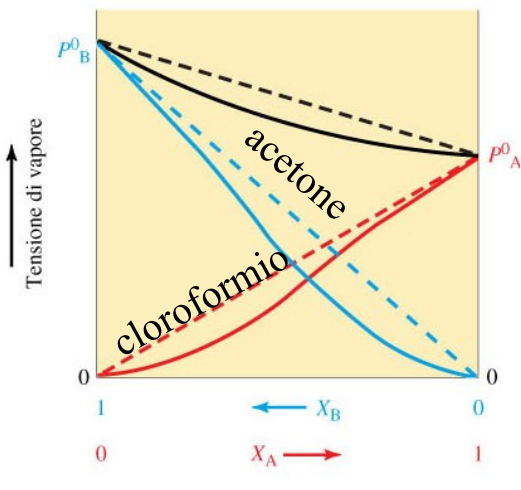
\includegraphics[width=6cm]{immagini/tensione_di_vapore_sol_esotermica.png}
    \end{figure}
\end{minipage}
\begin{minipage}{0.6\textwidth}
    Consideriamo una soluzione formata da acetone CH$_3$-CO-CH$_3$ e cloroformio CHCl$_3$.

    Le tensione di vapore del cloroformio puro è minore di quella dell'acetone puro. Ciò significa che a parità di temperatura la specie B è più volatile. Inoltre sperimentalmente si osserva che entrambi i componenti hanno tensioni di vapore minori di quelle previste dall'idealità, e quindi anche la soluzione avrà un comportamento che mostra un abbassamento della tensione di vapore.
\end{minipage}
\E inoltre conveniente, essendo un reazione che sprigiona calore, allontanare quest'ultimo, in quanto raffreddando il processo di dissoluzione viene facilitato.

La reazione sarà

$$\ce{A + B ->} \text{soluzione + calore}$$

Il motivo è che il calore può essere sia un reagente che un prodotto. Nel caso in cui sia un prodotto, nel momento in cui lo allontaniamo la reazione ne produrrà altro, ma questo comporterà la creazione di altra soluzione. In altre parole, allontanare i prodotti significa spostare verso destra quella reazione.
\subsection{Distillazione a P costante di soluzioni ideali}
Nei tre grafici precedenti avevamo la frazione molare in ascisse e la pressione in ordinate. Consideriamo adesso un grafico avente la frazione molare in ascisse e la temperatura in ordinate.

\begin{figure}[htp]
    \centering
    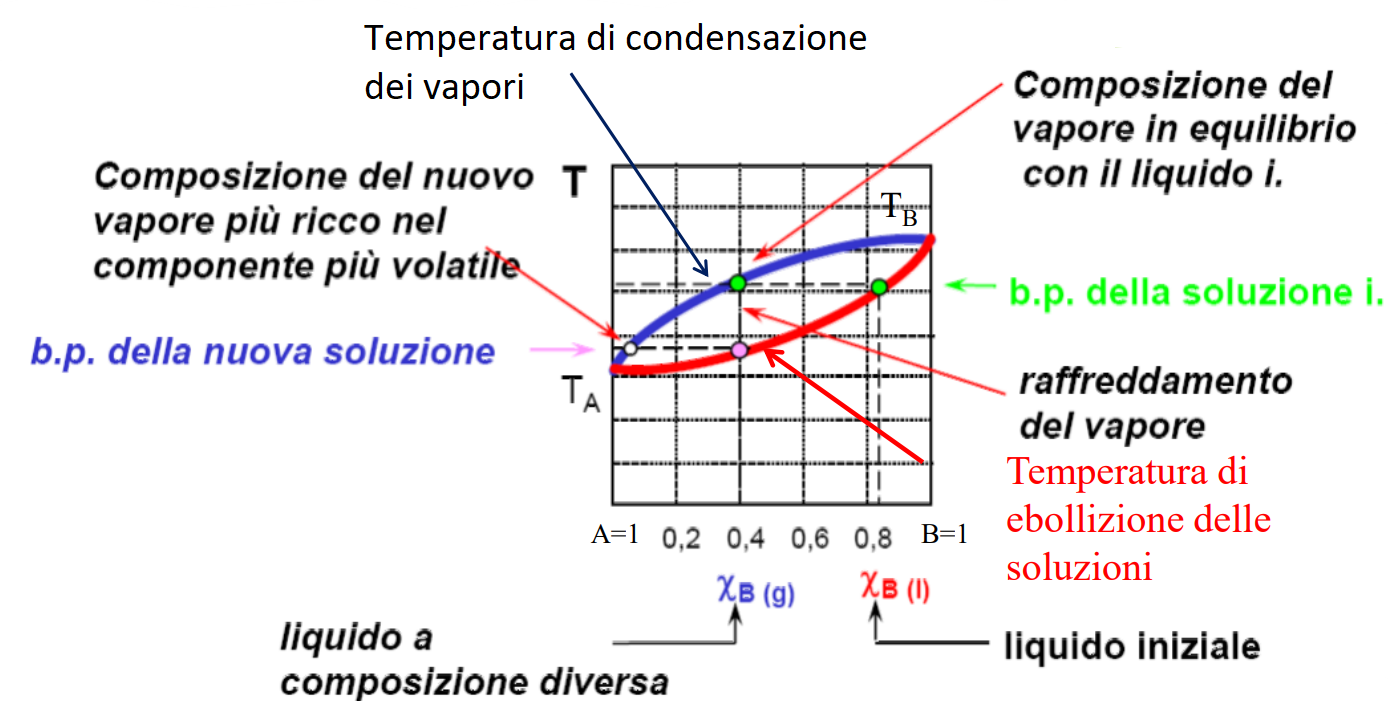
\includegraphics[width=15cm]{immagini/distillazione_ideale.png}
\end{figure}

Spesso in natura abbiamo delle soluzioni e il nostro obiettivo è separarle (ad es. il petrolio), ossia si vuole sfruttare la diversa volatilità di sostanze che si trovano in soluzione per separarle.

Il caso più semplice è quello di una soluzione formata da una specie A e una specie B. Graficamente avremo che in basso a sinistra la frazione molare di A è 1 e quella di B è 0, viceversa in basso a destra la frazione molare di B è 1 e quella di A è 0. Nei punti intermedi avremo invece tutte le infinite composizioni della miscela possibili.

Va da notare che i grafici sono sperimentali.

$T_A$ è la temperatura di ebollizione del componente A puro, $T_B$ quella del componente B puro.

Dal grafico si evince che B è meno volatile di A, infatti ha una temperatura di ebollizione più alta.

La linea rossa indica le diverse temperature di ebollizione delle varie soluzioni, quindi ogni soluzione AB avente la sua specifica composizione avrà una sua particolare temperatura di ebollizione.

La linea blu invece indica la temperatura di condensazione dei vapori aventi le diverse composizioni.

Il motivo per cui rappresentiamo queste due linee è che se vogliamo distillare l'obiettivo è quello di raccogliere poi il distillato e farlo condensare.

Supponiamo di avere una certa composizione della soluzione (nel disegno indicata dal punto verde sulla linea rossa) e iniziamo a riscaldare. La temperatura aumenterà fino a raggiungere la temperatura di ebollizione della soluzione, per cui la soluzione bolle, cioè la tensione di vapore ha eguagliato la pressione atmosferica (o in generale la pressione esterna). Inoltre da questo momento in poi fin quando  tutto il liquido non diventa vapore la temperatura non aumenta più. Allora si parla di \textit{calore latente di evaporazione}.

Dato che la soluzione sta bollendo abbiamo ottenuto dei vapori. Cosa abbiamo in fase vapore?

Ci si sposta orizzontalmente verso sinistra fino a trovare la curva blu. In questo modo la temperatura di condensazione del vapore è uguale alla temperatura di ebollizione, ma la composizione cambia: se raffreddiamo il vapore troveremo una composizione diversa da quella di partenza (indicata dal punto rosa sulla curva rossa).

Se riscaldiamo la nuova soluzione ottenuta per condensazione avremo una nuova temperatura di ebollizione. Se condensiamo il nuovo vapore dal grafico si evince che otterremo una soluzione composta quasi del tutto da A. Infatti per successive distillazioni si è in grado di ottenere A puro come distillato e B come residuo. Quindi se la soluzione ha comportamento ideale saremo in grado di separare, per successive distillazioni, i due componenti. In particolare il più volatile sarà nella fase vapore, il quale viene poi condensato; il meno volatile sarà nella fase liquida.

\E dunque possibile separare le soluzioni ideali nei loro componenti attraverso la distillazione. Il processo dovrà solo essere ripetuto perché di volta in volta i vapori saranno più ricchi nel componente più volatile.
\subsection{Distillazione di soluzioni reali}
Andiamo adesso a vedere cosa succede per soluzioni non ideali, cioè che deviano dalla legge di Raoult. Esse sono tutte quelle soluzioni per le quali le interazioni tra A e B sono o più deboli o più forti rispetto alle interazioni A-A e B-B, ossia quando $\Delta$H$>$0 o $\Delta$H$<$0. Anche in questo caso si ottengono grafici sperimentali.

\vspace{0.2cm}Consideriamo il caso in cui $\Delta$H$_{sol}<$0, cioè quello in cui la reazione è esotermica e quindi la soluzione emette calore.

Dal grafico si evince che la temperatura necessaria per far bollire e distillare ogni possibile soluzione si è alzata, quindi si deve fornire più energia. Il motivo è che le interazioni che si hanno nelle molecole in soluzione risultano essere più forti di quelle presenti tra le molecole nelle speci pure.

\begin{minipage}{0.4\textwidth}
    \begin{figure}[H]
        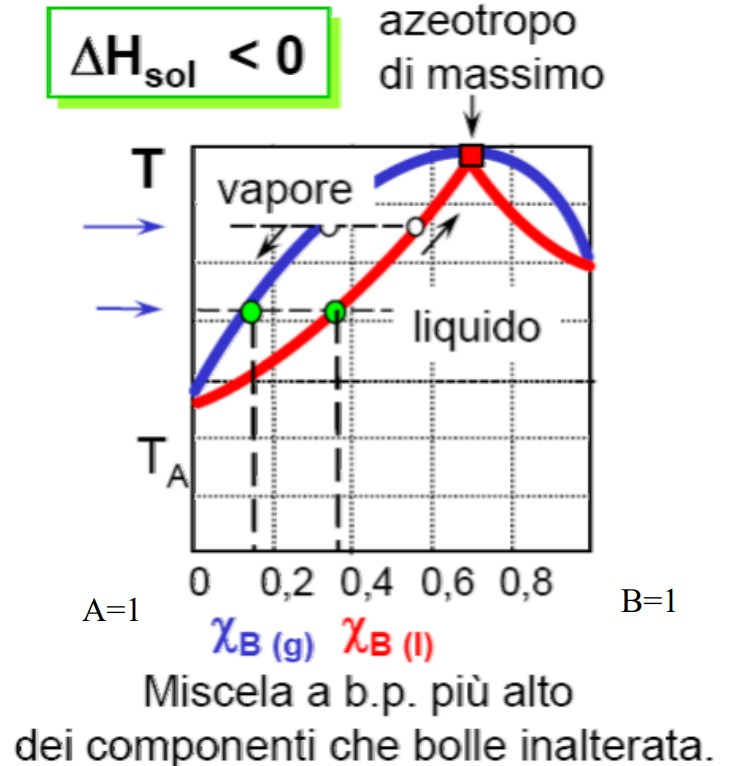
\includegraphics[width=6cm]{immagini/distillazione_esotermica.png}
    \end{figure}
\end{minipage}
\begin{minipage}{0.6\textwidth}
    \vspace{0.6cm}Presa una certa composizione, la riscaldiamo fino ad arrivare al punto sulla linea rossa che indica la temperatura di ebollizione. La soluzione inizierà a bollire e la composizione del vapore sarà ottenuta spostandoci orizzontalmente a sinistra. Si evince che nel vapore la quantità di A, rispetto a quella della soluzione liquida, è aumentata.

    Se A aumenta nella fase vapore significa che lo stiamo sottraendo alla fase liquida, quindi in quest'ultima avremo più B. Pertanto il vapore sta producendo A, mentre la soluzione si sta spostando a destra come composizione.
\end{minipage}

\vspace{0.2cm}Ci sarà un punto in cui la soluzione, cioè la fase liquida, raggiungerà la composizione corrispondente al quadrato rosso nel grafico. Tale punto è comune alla linea del liquido e a quella del vapore, ossia la composizione del liquido (che si sta arricchendo in B perché stiamo facendo evaporare A) diventa uguale alle composizione del vapore che distilleremo. A questo punto sarà inutile fare ulteriori distillazioni, perché si è arrivati alla \textbf{composizione azeotropica}, cioè si è formato un \textbf{azeotropo}, ossia una soluzione che bolle inalterata (cioè la composizione di liquido e vapore sono uguali).

Otterremo quindi l'azeotropo come residuo e A puro come distillato.

Abbiamo fatto un esempio in cui partivamo da una composizione a sinistra dell'azeotropo, adesso partiamo da una composizione a destra di questo.

In questo caso, dopo aver portato all'ebollizione la soluzione, la composizione del vapore si otterrà spostandoci orizzontalmente verso destra, cioè il vapore sarà più ricco in B. Se però sottraiamo B dalla soluzione, quest'ultima si arricchirà in A. In altre parole avremo B nella fase vapore e una soluzione avente composizione con meno B che quindi si sposta verso sinistra.

Con successive distillazioni avremo B puro come distillato e l'azeotropo come residuo.

Quindi, qualunque sia la composizione dalla quale partiamo, possiamo ottenere, a seconda se ci troviamo a sinistra o a destra dell'azeotropo, rispettivamente, A puro come distillato e l'azeotropo come residuo oppure B puro come distillato e ancora l'azeotropo come residuo, ossia si riesce a separare solo una parte di un componente e si può fino a quando non otteniamo in soluzione una composizione che è quella azeotropica, che ritroviamo nella fase vapore.

Questo è il problema per cui, ad esempio, per distillazione tra acqua e alcol non è mai possibile, pur essendo l'alcol più volatile, ottenere l'alcol "assoluto" cioè puro. Tuttavia l'alcol puro è comune in laboratorio. Come si fa?

Si distilla acqua ed alcol reiterando il processo fino a quando raggiungiamo l'azeotropo, per cui ci si deve fermare. Si prende allora questa soluzione (che non è più possibile separare nei suoi componenti) composta da tanto alcol e dalla poca acqua che non siamo riusciti a separare, e la si fa reagire con ossido di calcio. L'ossido assorbirà l'acqua residua diventando idrossido, quindi ora il problema sarà separare alcol e idrossido di calcio, che è un solido gelatinoso. Per fare ciò si adoperano altri metodi che eludono dai nostri studi.

\vspace{0.2cm}Consideriamo adesso una soluzione con $\Delta$H$>$0, cioè il processo di dissoluzione è endotermico e bisogna dunque fornire energia altrimenti la soluzione non si forma. Ciò significa che le interazioni tra A e B sono deboli rispetto a quelle che si esercitavano nei liquidi puri e infatti tutte le possibili soluzioni avranno temperature di ebollizione più basse.

\vspace{-0.2cm}\begin{minipage}{0.4\textwidth}
    \begin{figure}[H]
        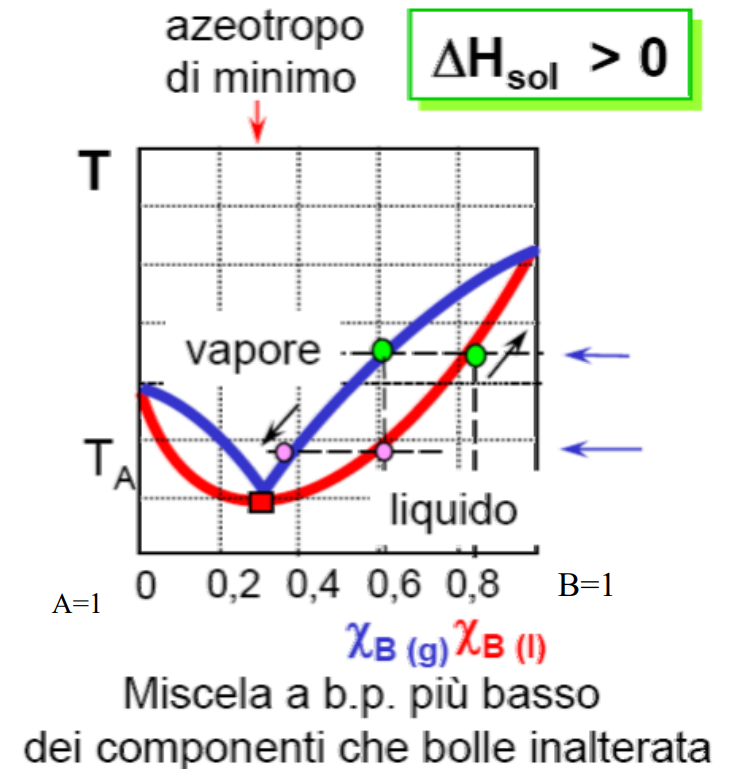
\includegraphics[width=6cm]{immagini/distillazione_endotermica.png}
    \end{figure}
\end{minipage}
\begin{minipage}{0.6\textwidth}
    \vspace{0.6cm}Immaginiamo di essere a destra dell'azeotropo e di avere una certa composizione. Riscaldiamo la soluzione fino a quando inizia a produrre vapore, il quale avrà una diversa composizione (più a sinistra). Condensandola troviamo una nuova soluzione, più vicina all'azeotropo.

    Quindi succede il contrario del caso precedente, cioè mentre prima il vapore ci dava A puro o B puro a seconda che ci trovassimo a destra o a sinistra dell'azeotropo, ora invece sarà il vapore ad avvicinarsi alla composizione azeotropica, pertanto stavolta avremo l'azeotropo come distillato e il componente come puro come residuo.
\end{minipage}

\vspace{0.2cm}In sintesi, se ci troviamo alla destra dell'azeotropo avremo l'azeotropo come distillato e B puro come residuo, se ci troviamo alla sua sinistra otterremo l'azeotropo come distillato e A puro come residuo.

\vspace{0.2cm}Recap: discutendo la legge di Raoult, valida per soluzioni ideali, abbiamo visto che la tensione di vapore di queste è funzione della loro composizione. Si hanno quindi dei diagrammi con frazione molare sulle ascisse e tensione di vapore sulle ordinate. Questi sono grafici validi per temperature fissate.

Ci siamo chiesti se, presa una soluzione formata da due componenti, sia possibile separare i due liquidi. Ciò è possibile solo per soluzioni ideali.

Abbiamo allora considerato dei grafici a pressione costante, con la frazione molare sulle ascisse e la temperature sulle ordinate. Da essi si evince che qualunque sia la composizione iniziale è possibile ottenere, per successive distillazioni, i componenti puri.

Viceversa per le soluzioni non ideali non è possibile ottenere entrambi i componenti del tutto puri, ma di norma si ottiene uno dei due puro mentre l'altro si ottiene con una composizione detta azeotropica.

Abbiamo affrontato il caso in cui l'entalpia di mescolamento $\Delta$H sia positiva e il caso in cui sia negativa. Queste soluzioni sono dovute al fatto che le interazioni tra le molecole di A e quelle di B risultano essere diverse da quelle che si esercitano nelle speci pure (per diverse si intende che sono più forti o più deboli). Per entrambi i casi abbiamo poi visto cosa succede se ci troviamo a sinistra o a destra dell'azeotropo. Si trova che distillando il vapore sarà più ricco in una componente e il residuo sarà di conseguenza più ricco nell'altra. Quest'ultimo tende ad andare verso la composizione azeotropica, in cui la miscela "non distilla più", nel senso che il vapore avrà la stessa composizione del liquido, quindi sarà inutile fare l'operazione di distillazione.